\chapter{Análise do Problema}
\section{Descrição do Problema}
O principal problema a ser resolvido pela turma B é garantir que as medições de temperatura e pressão durante a execução de testes com combustão sejam confiáveis.

Em um grupo com alunos de Engenharias distintas, é necessário usar uma ferramenta para melhorar a compreensão do projeto. Para a documentação do problema foi escolhido o fishbone (diagrama de Ishikawa). Segue abaixo o resultado:

\begin{figure}[!htb]                                                               
   \centering                                                                      
   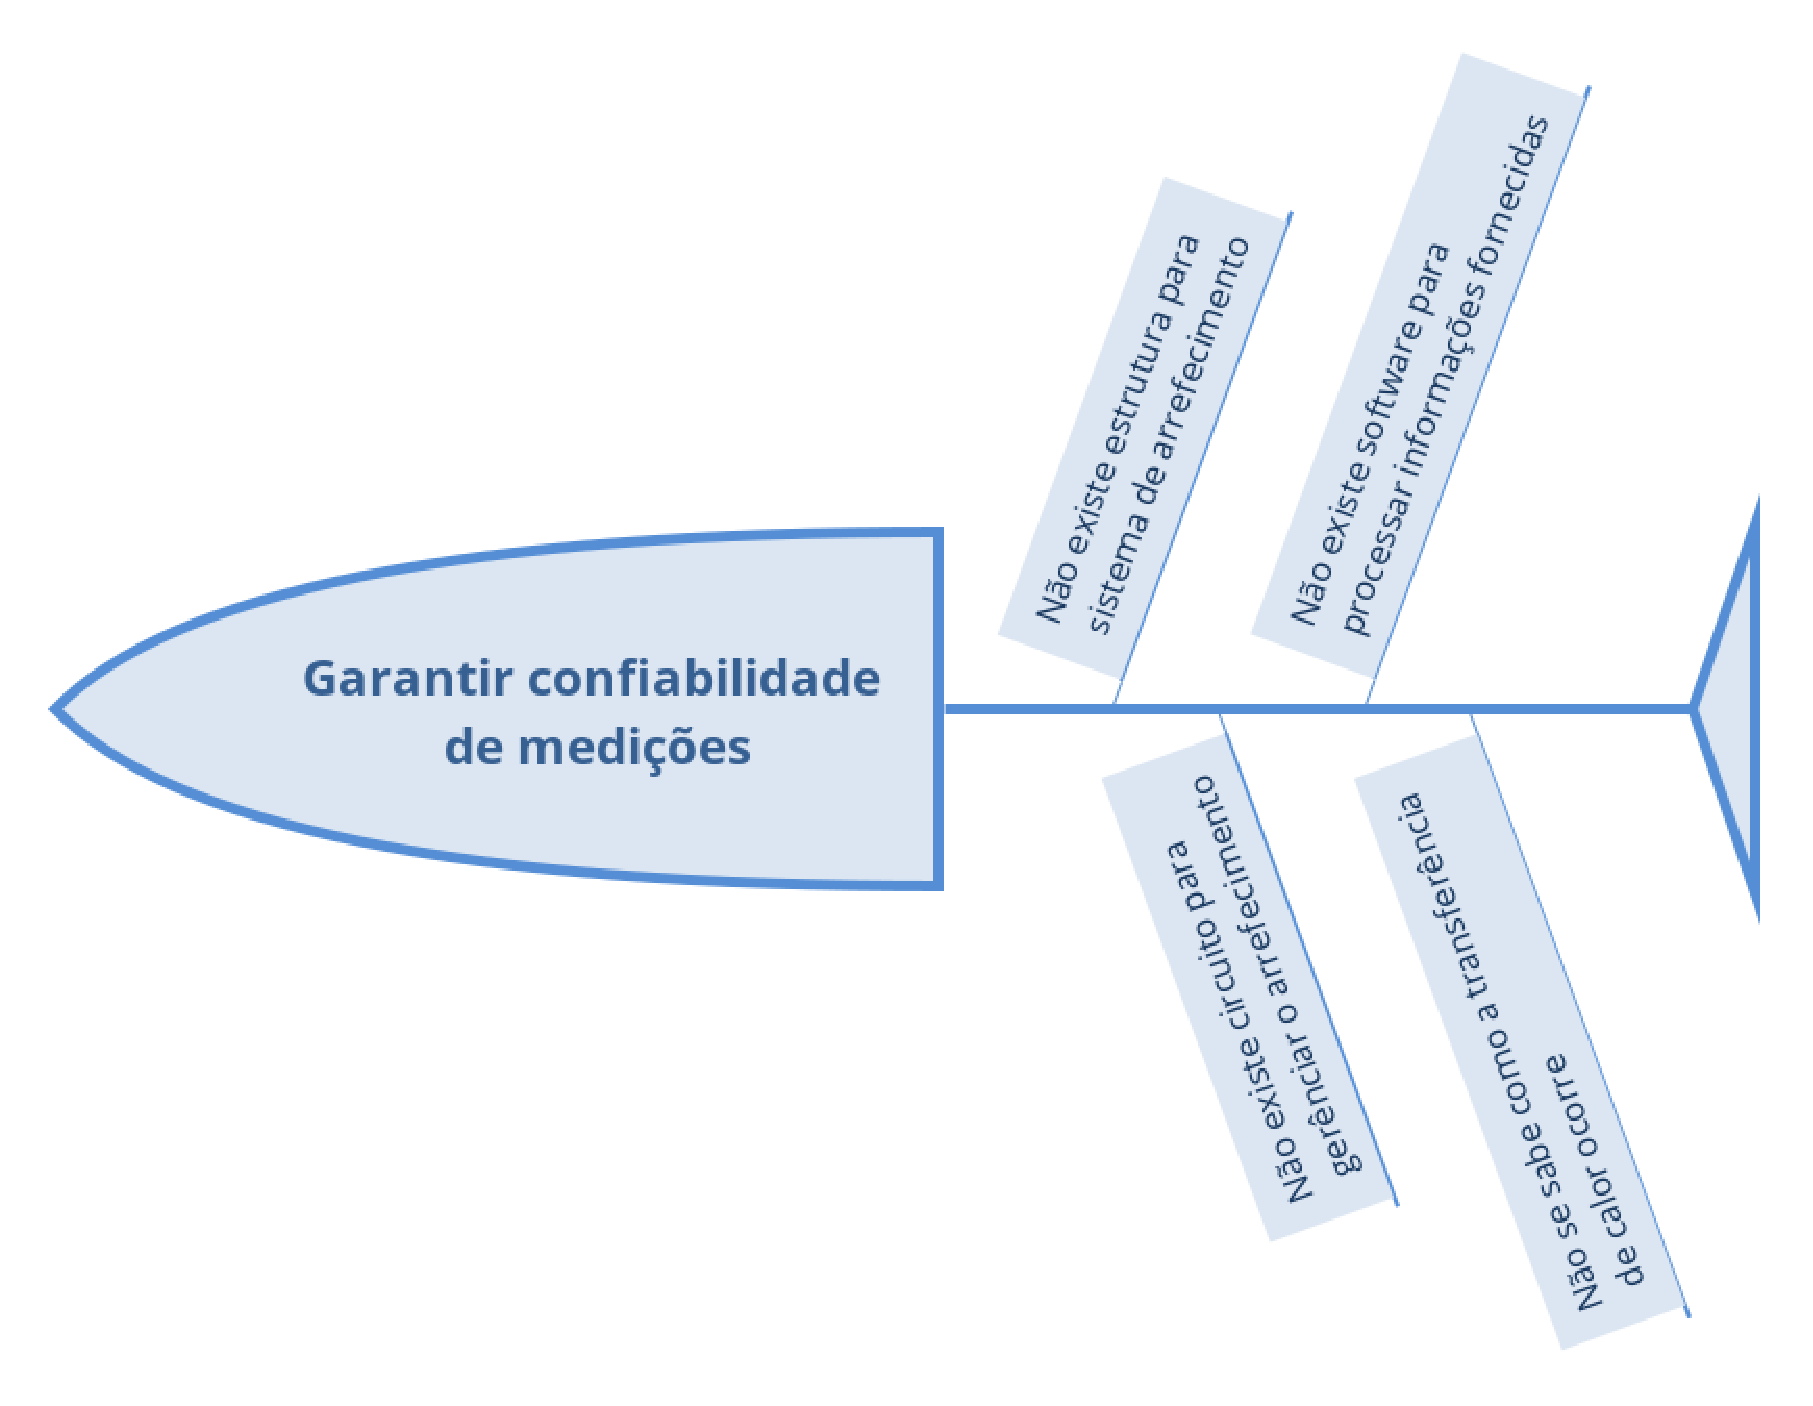
\includegraphics[width=15cm, keepaspectratio=true]{figuras/fishbone.eps}
   \caption{Visão de dependência entre as tarefas e prazos}                        
\end{figure}

\section{Requisitos}
Com a definição do problema a ser atacado com o projeto, foi necessário executar a elicitação dos requisitos. Para garantir que todas as engenharias relacionadas, pudessem ter compreensão dos requisitos, os mesmos foram documentados usando os conceitos de Engenharia de requisitos que os divide em 3 camadas:

\begin{enumerate}
	\item Requisitos Raiz
		\begin{enumerate}[start=1,label*={\arabic*}]
			\item Medir calor e pressão com confiabilidade
		\end{enumerate}
	
	\item Requisitos de Negócio
		\begin{enumerate}[start=2,label*={\arabic*}]
			\item Utilizar apenas produtos de bancada
			\item Ter custo inferior à 2000 euros
			\item Ser implementável no contexto da FGA
		\end{enumerate}

	\item Requisitos de sistema
		\begin{enumerate}[start=3,label*={\arabic*}]
			\item Garantir controle do usuário durante a execução de testes
			\item Resfriar os equipamentos de medições com eficiência
			\item Garantir a confiabilidade dos dados recebidos pelo sistema
			\item Ser implementado com o software LabView
		\end{enumerate}
\end{enumerate}

Estes requisitos geraram atividades que foram apresentadas no primeiro Ponto de Controle, estas atividades foram divididas entre os times de acordo com as suas áreas.

Ao final da disciplina, é esperado que todos os requisitos sejam satisfeitos, e assim garantir que o projeto foi um sucesso.
